\documentclass[journal,transmag]{IEEEtran}
    \usepackage{algorithm}
    \usepackage{graphicx}
    \usepackage{verbatim}
    \usepackage{pythonhighlight}
    \usepackage{listings}

    \hyphenation{op-tical net-works semi-conduc-tor}
    \begin{document}
    \title{ Analysis and Comparison of Brute-Force and Genetic Algorithm methods
        on Traveling Salesman Problem }

    \author{ \IEEEauthorblockN{Onur Temizkan} \IEEEauthorblockA{ Department of
        Computer Engineering, Izmir Institute of Technology, Urla / Izmir /
        Turkey } }

    \markboth{Optimization Methods Term Project, Onur Temizkan, June 2018}{}%

    \IEEEtitleabstractindextext{%
    \begin{abstract}
        \textit{ Abstract: Traveling Salesman Problem (TSP) is a common
            NP-Complete problem in Computer Science and Optimization. Thus,
            there is no known way to solve it in polynomial time at the time of
            this writing. In this report,  Genetic algorithm
            approach will be analyzed on TSP and compared with Brute-Force Search method. }
    \end{abstract}

    \begin{IEEEkeywords}
    traveling salesman problem, optimization, genetic algorithm, TSP,
    combinatorics.
    \end{IEEEkeywords}}

    \maketitle
    \IEEEdisplaynontitleabstractindextext \IEEEpeerreviewmaketitle

    \section{Introduction}

    \IEEEPARstart{I}{n} this report, The performance of a genetic algorithm
    implementation will be analyzed, onto Traveling Salesman Problem to find
    the optimum path to traverse a multi-node undirected and weighted graph. On
    the other side, to measure the pros / cons of the Genetic Algorithms,
    brute-force method will also be applied on the same problem. The problem
    definitions and solutions are implemented in Python.

    \section{Problem Definition}

    For this research, the problem is defined as a \textit{undirected graph}
    with \textit{N} nodes. There are edges with several weights between those nodes. In
    TSP analogy, the nodes represent cities, and edges represent paths between
    those cities. Edge weights, represent the distances between two cities. A
    route is valid if the salesman start traveling from a given node, visit all
    cities once, and return back to the starting city.

    Since the graph is not necessarily a \textit{complete graph}, the algorithm
    should check next available nodes from the node at a single time to create
    the route. All nodes should be visited once. So the implementation should be
    aware of the possible circular routes and should avoid them.

    Moreover, since the graph edges are weighted by definition, the algorithms we
    implement should select from possible routes in awareness of costs.

    The TSP that will be solved is shown in Figure \ref{fig:tsp-problem}

    \begin{figure}[H]
        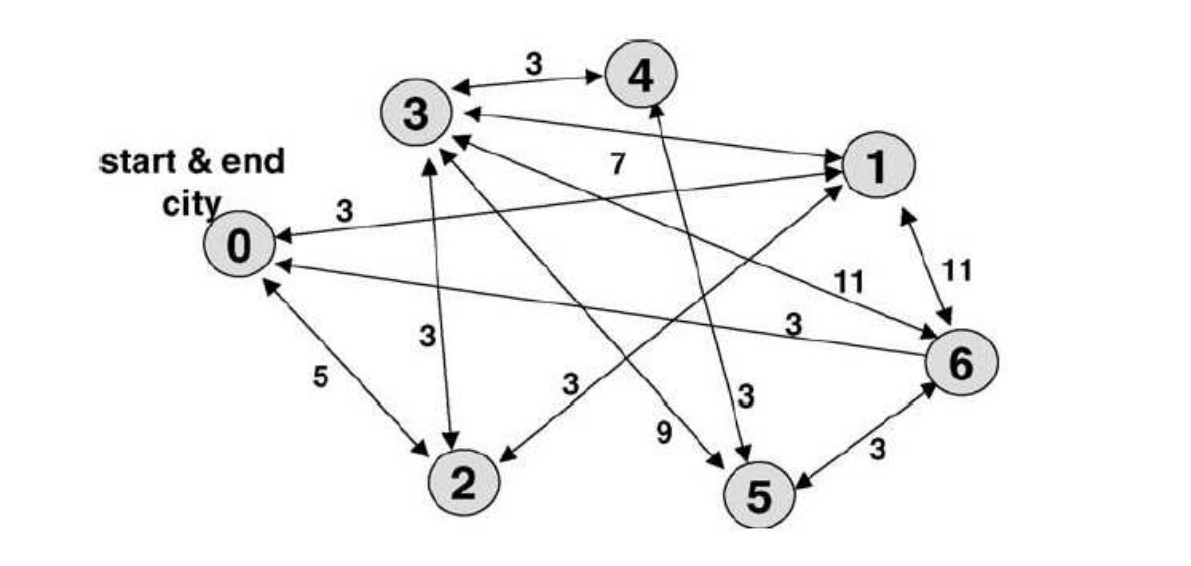
\includegraphics[width=\linewidth]{tsp.png}
        \caption{TSP to be solved}
        \label{fig:tsp-problem}
    \end{figure}


    \section{Methods}

    In this experiment, two different methods will be applied to the same problem.

    \subsection{Brute-Force Search}

    Brute-Force Search solves this problem in an inefficient but a definite way.
    To find the best route, Brute-Force Search checks all possible path
    permutations without any specific condition or restriction. While checking
    routes, it stores and updates the shortest route from the start of the
    execution. When the checks are finished, the shortest route is the last
    route stored. Since it checks all possible routes, it makes sure that the
    returned result is the best possible solution. This implementation is very
    memory-efficient because only thing that is stored, is the shortest path and
    its size. But it's also very time inefficient because all the path
    combinations are tried.

    \subsection{Genetic Algorithm}

    Solving the problem with a Genetic Algorithm is more efficient but
    indefinite. This is because in a Genetic Algorithms, it's not necessary to check all
    possible routes. Instead, evolving a set of routes is tried to create a
    better route. GA approach is an iterative method which is based on the
    natural selection mechanism of evolution. Since natural selection
    \textit{-thus evolution} doesn't have a stopping point, Genetic Algorithms
    do not have a strict finishing point. So it's presumed that there can always be
    a better solution at the any state of the algorithm execution, and a
    stopping condition should be chosen.

    \begin{algorithm} % enter the algorithm environment
        \textit{1.} Create a population with \textit{N} random routes. \\
        \textit{2.} Select the best \textit{k} routes \\
        \textit{3.} combine / match the selected routes to create an ancestor
        route. \\
        \textit{4.} Mutate that ancestor node \textit{N-1} times to create a new
        generation with N new routes. \\
        \textbf{Repeat} steps \textit{2} to \textit{4}, \\
        \textbf{Until} the best route hasn't been changing for x generations \\
        \textit{5.} Return the best route and its length.


        \caption{Genetic Algorithm on TSP} % give the algorithm a caption
        \label{alg2} % and a label for \ref{} commands later in the document

    \end{algorithm}

    \section{Implementation}

    The code \cite{code_repository} of both Brute-Force and Genetic Algorithm
    approaches are implemented in Python. We tried to keep the code simple by
    removing any nonessential parts such as status logs. This also helped to
    measure and compare the performances since there are almost no avertible
    computational cost in any of those two implementations.

    Python definition and representation of the TSP is shown below in Figure
    \ref{fig:data-definition}. Each member of \texttt{PATH\_DEF}, represent a city
    with its connections to other cities. The connections are represented by a
    list of tuples. The first element of each tuple represents the connected
    city, and the second one represents the distance to that city.


    \begin{figure}[H]
        \begin{python}
PATH_DEF = {
    0: [(1, 3), (2, 5), (6, 3)],
    1: [(0, 3), (2, 3), (3, 7), (6, 11)],
    2: [(0, 5), (1, 3), (3, 5)],
    3: [(1, 7), (2, 3), (4, 3), (5, 9), (6, 11)],
    4: [(3, 3), (5, 3)],
    5: [(3, 9), (4, 3), (6, 3)],
    6: [(0, 3), (1, 11), (3, 11), (5, 3)]
}
        \end{python}
        \caption{TSP Data Definition}
        \label{fig:data-definition}
    \end{figure}

    An excerpt from Brute-Force implementation is given below. This
    implementation first find all the possible routes in the problem definition,
    then calculates the path sizes of each route. While doing that, it stores
    the shortest route at the time of execution. After traversing all the
    routes, it returns the best route found and its distance.
    \begin{figure}[H]
        \begin{python}
def trav_salesman():
    for point in PATH_DEF:
        find_all_paths([point])

    min_length = inf
    min_path = None

    for path in all_paths:
        path_length = calc_path_length(path)
        if path_length < min_length:
            min_path = path
            min_length = path_length
        \end{python}
        \caption{Brute Force Implementation}
    \end{figure}

    Genetic algorithm implementation is a little bit more complex. It first
    creates a random population. Then until a limit of generations, it generates
    a new populations using fittest paths. An excerpt from that implementation
    can be found in Figure 4.

    Since our test example is an incomplete undirected graph, our genetic implementation
    is based on specifically for that kind of graphs, another implementation for
    complete graphs can also be found in given repository. \cite{code_repository}

    \begin{figure}[H]
        \begin{python}
def trav_salesman():
    population = pre_populate()

    for i in range(MAX_GENERATIONS):
        fittest = get_fittest(population)
        (fittest_path, fittest_length) = fittest

        all_generation_fittest_lengths.append(
            fittest_length
        )
        all_generation_average_lengths.append(
            get_average(population)
        )
        all_generation_worst_lengths.append(
            get_worst(population)[1]
        )

        population = populate(fittest_path)
        \end{python}
        \caption{Genetic Algorithm Implementation}
    \end{figure}

    \section{Results}  \label{results}
    \subsubsection{First Trial}
    In the first implementations of these two algorithms, the results were
    interesting. Genetic Algorithm took more time than Brute-Force
    implementation which was unexpected. The results are shown in
    Table I.

    \begin{table}[H]
        \begin{center}
            \begin{tabular}{| l | l | l |}
            \hline
            & Brute Force & Genetic Algorithm \\ \hline
            Iters / Gens & 102 & 7 \\ \hline
            Path & [0, 6, 5, 4, 3, 2, 1] & [3, 2, 1, 0, 6, 5, 4] \\ \hline
            Distance & 18 & 18 \\ \hline
            Time (sec.) & 0.00134 & 0.0024 \\
            \hline
            \end{tabular}
        \end{center}
        \caption{Compared Execution Results of First Implementation}
    \end{table}

    The reason of this would be the mutation logic and sample size selection.
    Also since the used problem size was very small, that implementation
    performed worse than brute-force implementation.

    The Genetic Algorithm implementation had a mutation logic which created a
    significant computational overhead. This overhead may become negligible in
    larger size problems but in this case, traversing all possible routes in
    Brute-Force implementation became less costly than these logic in Genetic
    Algorithm logic.

    Also as will be stated in \ref{second-trial}, this implementation didn't
    have any `Crossover' logic, which might be the source of the performance
    problem.

    So, the implementation should had been changed. What should had been tried is,
    keeping the mutation logic -\textit{of course} but making it more efficient
    for the algorithm to finish with less generations, thus earlier.
    \pagebreak

    \subsubsection{Second Trial} \label{second-trial}
    A new implementation with updated sample size and changed mutation logic,
    gave better results.

    The things that had changed were instead of mutating the best route in each
    generation while creating the new generation, the best \textit{N}
    generations are combined to create the new one, this implementation is
    actually the correct implementation of Genetic Algorithms. In the first
    implementation `Crossover', which is an important step of Genetic Algorithms
    had been skipped. This implementation had Crossover step and kept the
    mutation logic.

    The problem about the Crossover implementation on this problem was, since
    the graph is not fully connected, the result of crossover / and its
    mutations could be invalid routes. After applying crossover and also
    mutations, a validation had needed. If a route hadn't pass those
    validations, crossovers or mutations had to be repeated until finding a
    valid route.

    Although this implementation seems to have more computational overhead, it
    finds the shortest path in less generations. So this implementation worked
    much better than its predecessor. \\

    The new results are shown in Figure 5 and Table II.

    \begin{figure}[H]
        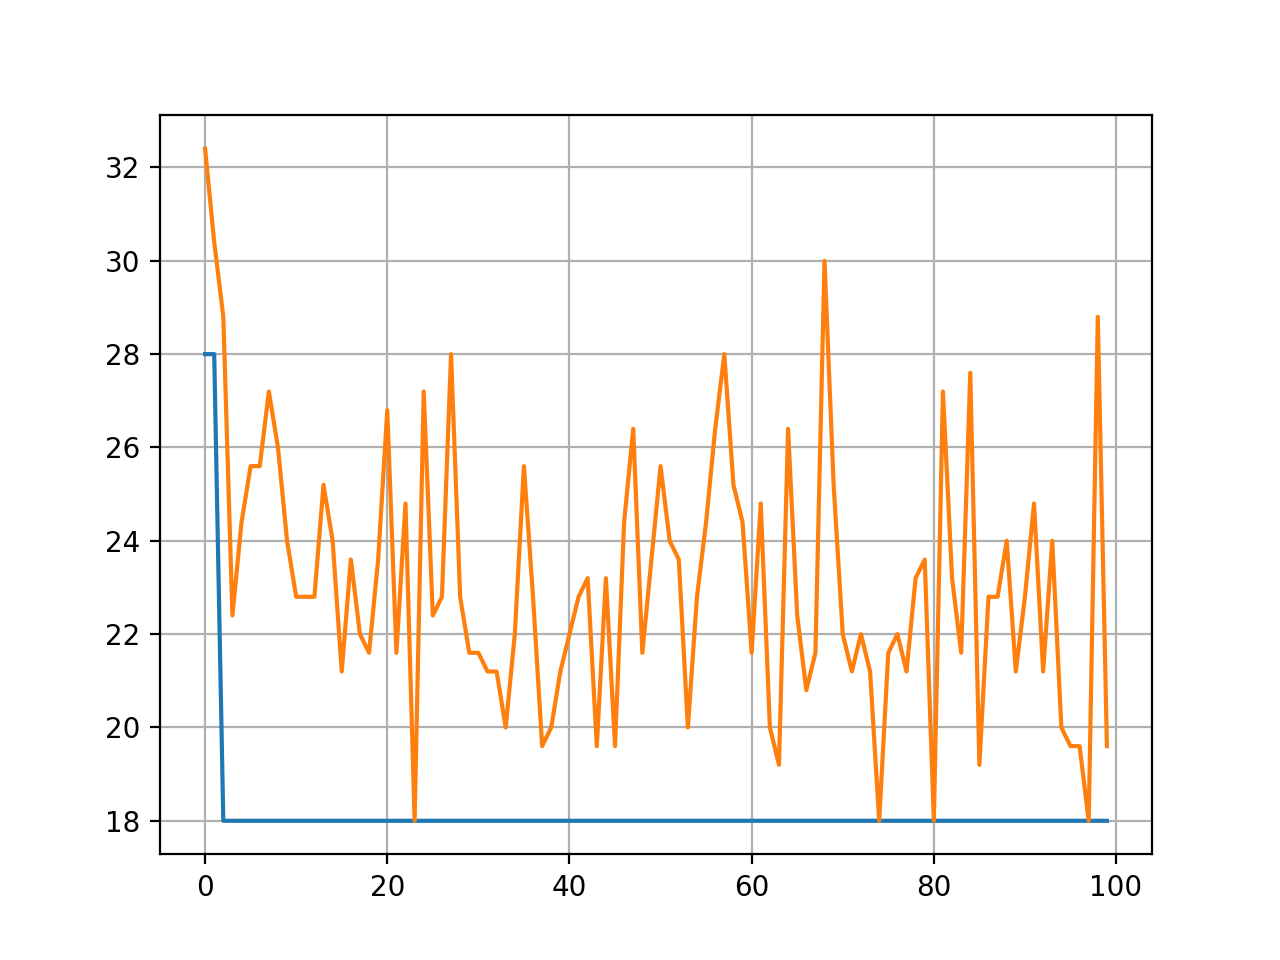
\includegraphics[width=\linewidth]{new-results.png}
        \caption{
            New results showing best route sizes in a generation in blue, and
            mean size of a generation in orange.
        }
        \label{fig:new-results}
    \end{figure}

    \begin{table}[H]
        \begin{center}
            \begin{tabular}{| l | l | l |}
            \hline
            & Brute Force & Genetic Algorithm \\ \hline
            Iters / Gens & 102 & 2 \\ \hline
            Path & [0, 6, 5, 4, 3, 2, 1] & [3, 2, 1, 0, 6, 5, 4] \\ \hline
            Distance & 18 & 18 \\ \hline
            Time (sec.) & 0.00134 & 0.00037 \\
            \hline
            \end{tabular}
        \end{center}
        \caption{Compared Execution Results of Second Implementation}
    \end{table}

    As can be seen, the new implementation of Genetic Algorithm Solution, the
    execution time got smaller and the result is found in the second generation.
    Also interestingly, the found solution of the Genetic Algorithm
    implementation is exactly the same as the first implementation results.

    \pagebreak

    \section{Conclusion}

    Genetic Algorithm approach works very well on Traveling Salesman Problem.
    That approach significantly reduced the number of visited routes to find the
    optimal route, comparing with the Brute-Force Search. Although, our sample
    problem is not so big, it reduced the execution time in a significant
    amount. When the problem gets bigger, the execution time benefits can be
    much more significant.

    Also, as stated in \ref{results}, the implementation is very important for
    the performance of the Genetic Algorithm. The performance measures can
    differ a lot with simple optimizations on implementation decisions.

    Giving directions to a searching quest of an optimal path should be almost
    every time better than just searching blindly. But in the sense of Genetic
    Algorithms the given directions seems to be even more accurate, providing
    that the correct solution is found in just two generations in our second
    implementation in \ref{second-trial}.

    To summarize, given the results of this experiment, Genetic Algorithms seem
    to be good solutions on NP-Complete problems. But since this experiment
    doesn't compare Genetic Algorithms with other possible solvers such as
    `Linear Programming', `Nearest Neighbour', `Simulated Annealing' and
    others, what is the best approach for these kind of problems cannot be
    stated.

    Note that this implementation is only a solution
    for incomplete graph based TSPs. For other TSP domains like coordinate
    systems, other implementations and logic should be applied. A sample
    implementation of these kind of problems can also be found in
    \cite{code_repository}.

    \ifCLASSOPTIONcaptionsoff
      \newpage
    \fi

    \begin{thebibliography}{1}

    \bibitem{code_repository}
    http://github.com/onurtemizkan/tsm-genetic-algorithm
    \end{thebibliography}

    \end{document}
